\section{Exercise 2}
Với mạch sau, học sinh sắp xếp lại mạch để làm rõ cấu trúc liên kết nối tiếp và/hoặc song song của nó. Sau đó, áp dụng kiến thức đã học để tìm điện trở tương đương
giá trị giữa hai đầu mạch A và F. Cuối cùng, thực hiện mô phỏng để kiểm tra xem
dòng điện qua toàn mạch được tính toán chính xác.\\
\begin{figure}[!htbp]
\centering
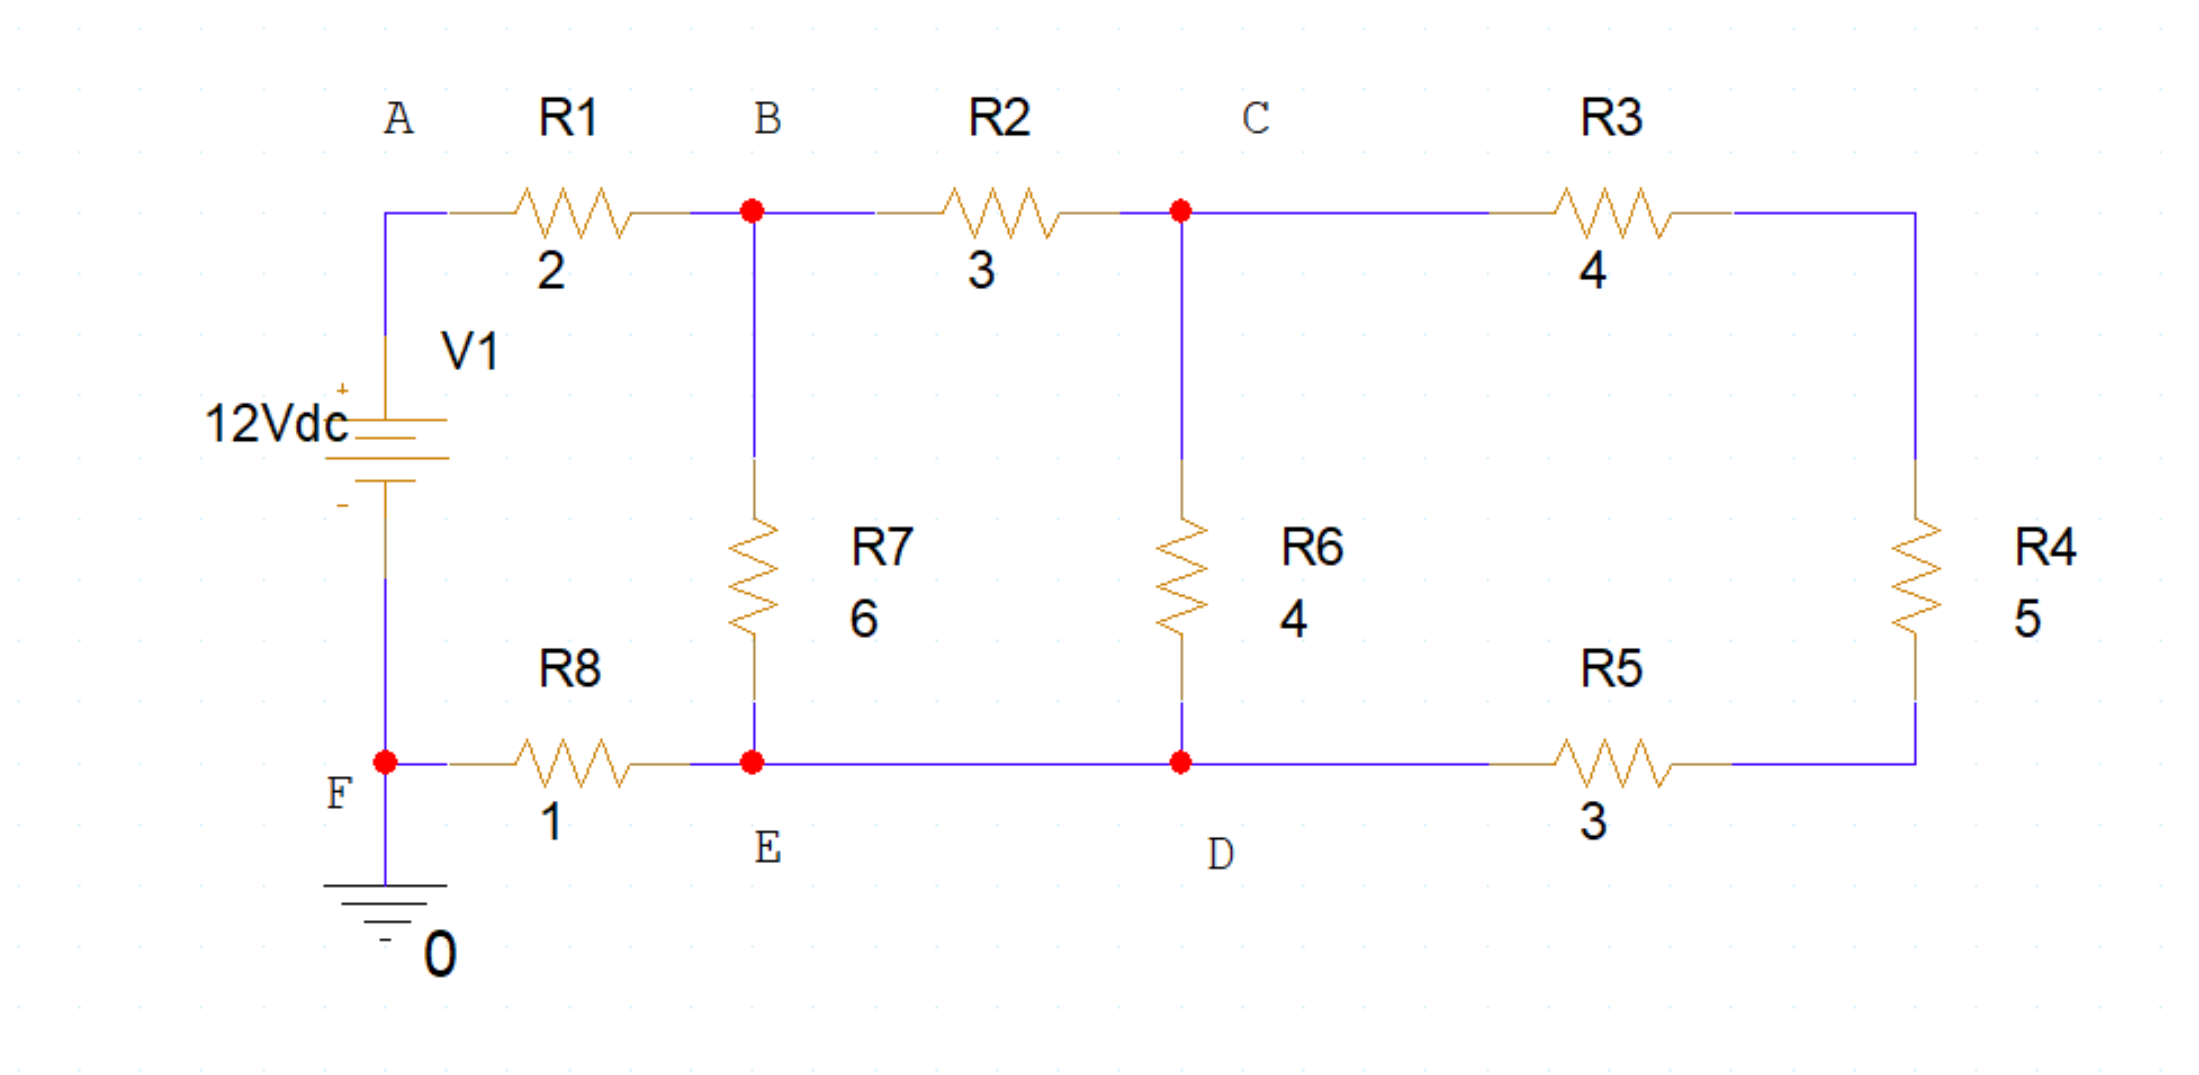
\includegraphics[width=1\textwidth]{graphics/ex2/f1.png}
\caption{Tìm giá trị điện trở tương đương giữa hai cực A và F}
\end{figure}
\subsection{Sắp xếp lại mạch}
\begin{figure}[!htbp]
    \centering
    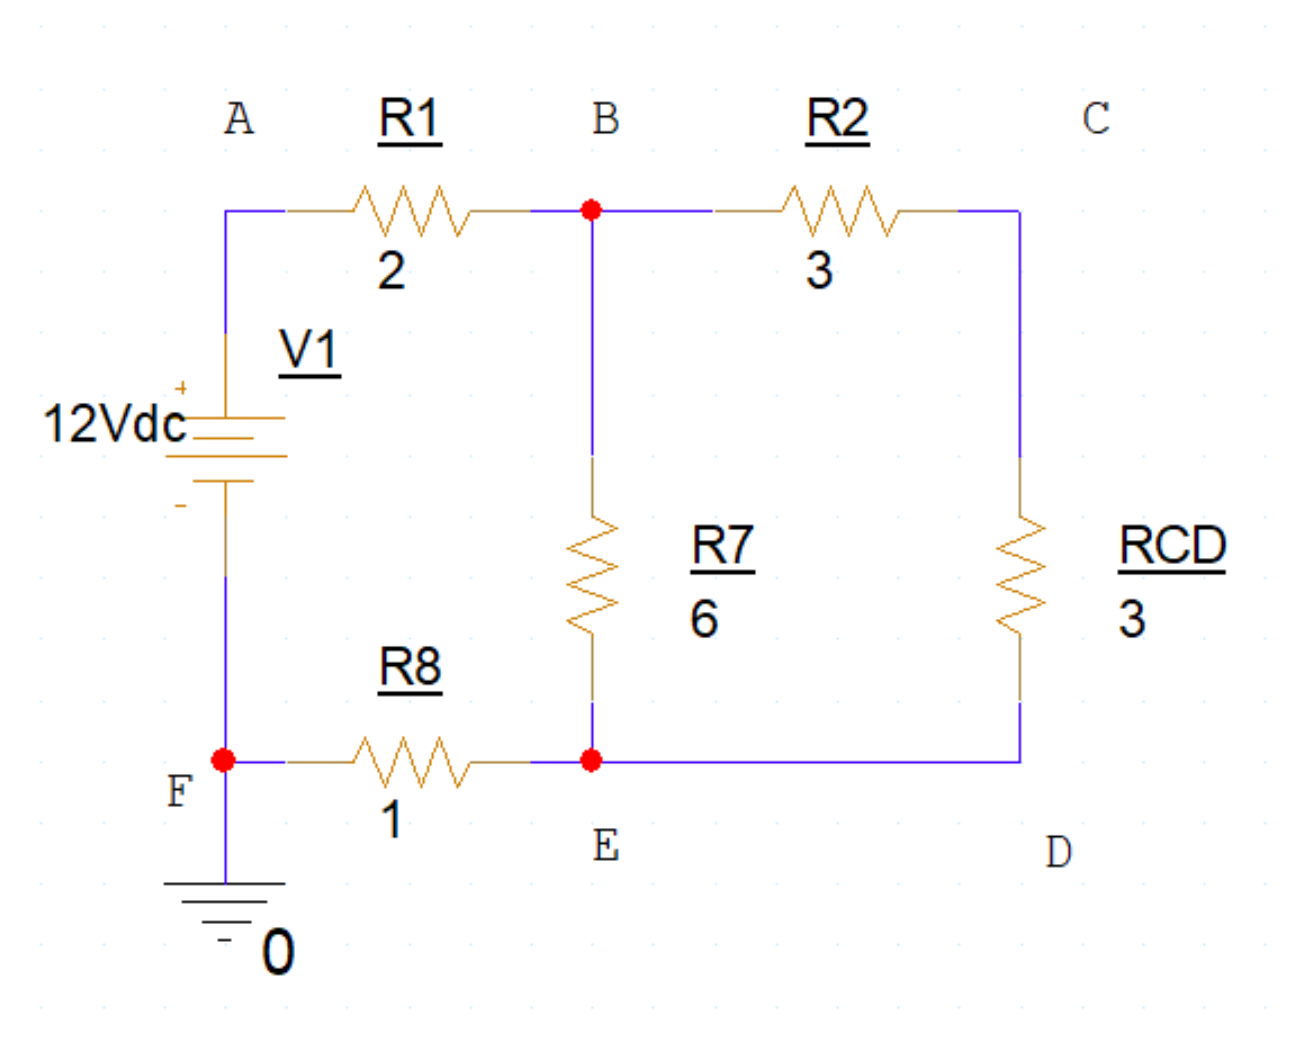
\includegraphics[width=0.6\textwidth]{graphics/ex2/f4.png}
    \caption{Thay \(R_3, R_4, R_5\) và \(R_6\) thành \(R_{CD}\) (\((R_3 nt R_4 nt R_5)//R_6\))}
\end{figure}    
\begin{figure}[!htbp]
    \centering
    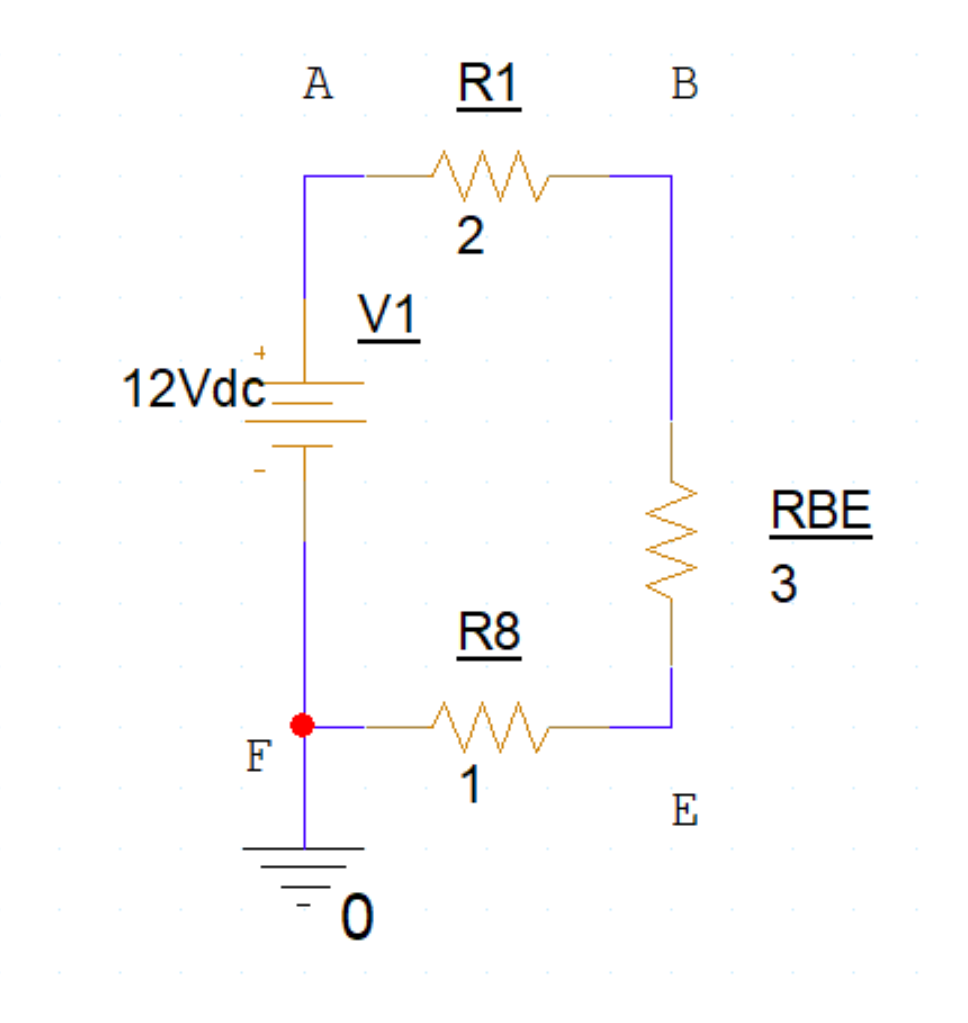
\includegraphics[width=0.4\textwidth]{graphics/ex2/f5.png}
    \caption{Thay \(R_{CD}, R_2, R_7\) thành \(R_{BE}\) (\((R_2 nt R_{CD})// R_7\) )}
\end{figure}
\begin{figure}[!htbp]
    \centering
    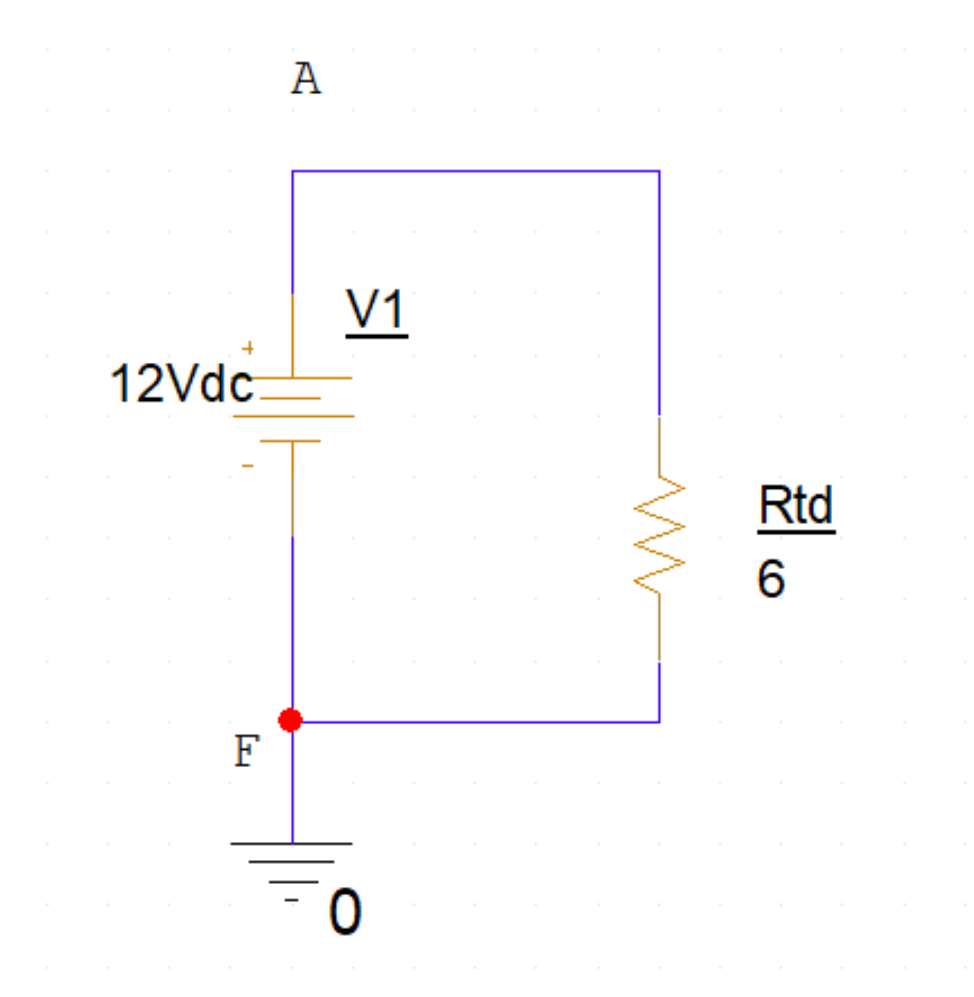
\includegraphics[width=0.4\textwidth]{graphics/ex2/f3.png}
    \caption{Thay \(R_{BE}, R_1, R_8\) thành \(R_{td}\) (\(R_{BE} nt R_1 nt R_8\))}
\end{figure}
\newpage
\subsection{Tính toán}
\textbf{Quy ước}:\\
Điện trở tương đương giữa hai đầu A và B của đoạn mạch chỉ chứa R1, R2, R3 và R4 có thể được gọi tên \(R_{AB \_ 123}\)
\begin{itemize}
\item Tính \(R_{CD}\)\\\(R_3 nt R_4 nt R_5 \rightarrow R_{345} = R_3 + R_4 + R_5 = 4 + 5 + 3 = 12 \Omega\)\\ \(R_{345} // R_6 \rightarrow \frac{1}{R_{CD}} = \frac{1}{R_{345}} + \frac{1}{R_6} = \frac{1}{12} + \frac{1}{4} \rightarrow R_{CD} = 3 \Omega\)
\item Tính \(R_{BE}\)\\\((R_{CD} nt R_2)//R_7 \rightarrow \frac{1}{R_{BE}} = \frac{1}{R_{CD} + R_2} + \frac{1}{R_7} = \frac{1}{3 + 3} + \frac{1}{6} = \frac{1}{3} \rightarrow R_{BE} = 3 \Omega\)
\item Tính \(R_{AF}\)\\\(R_1 nt R_{BE} nt R_8 \rightarrow R_{AF} = R_1 + R_{BE} + R_8 = 2 + 3 + 1 = 6 \Omega\)
\item Tính \(I_{AB}\)\\\(I_{AB} = I = \frac{V_1}{R_{AF}} = \frac{12}{6} = 2 A\)
\end{itemize}
\subsection{Mô phỏng}
\begin{figure}[!htbp]
    \centering
    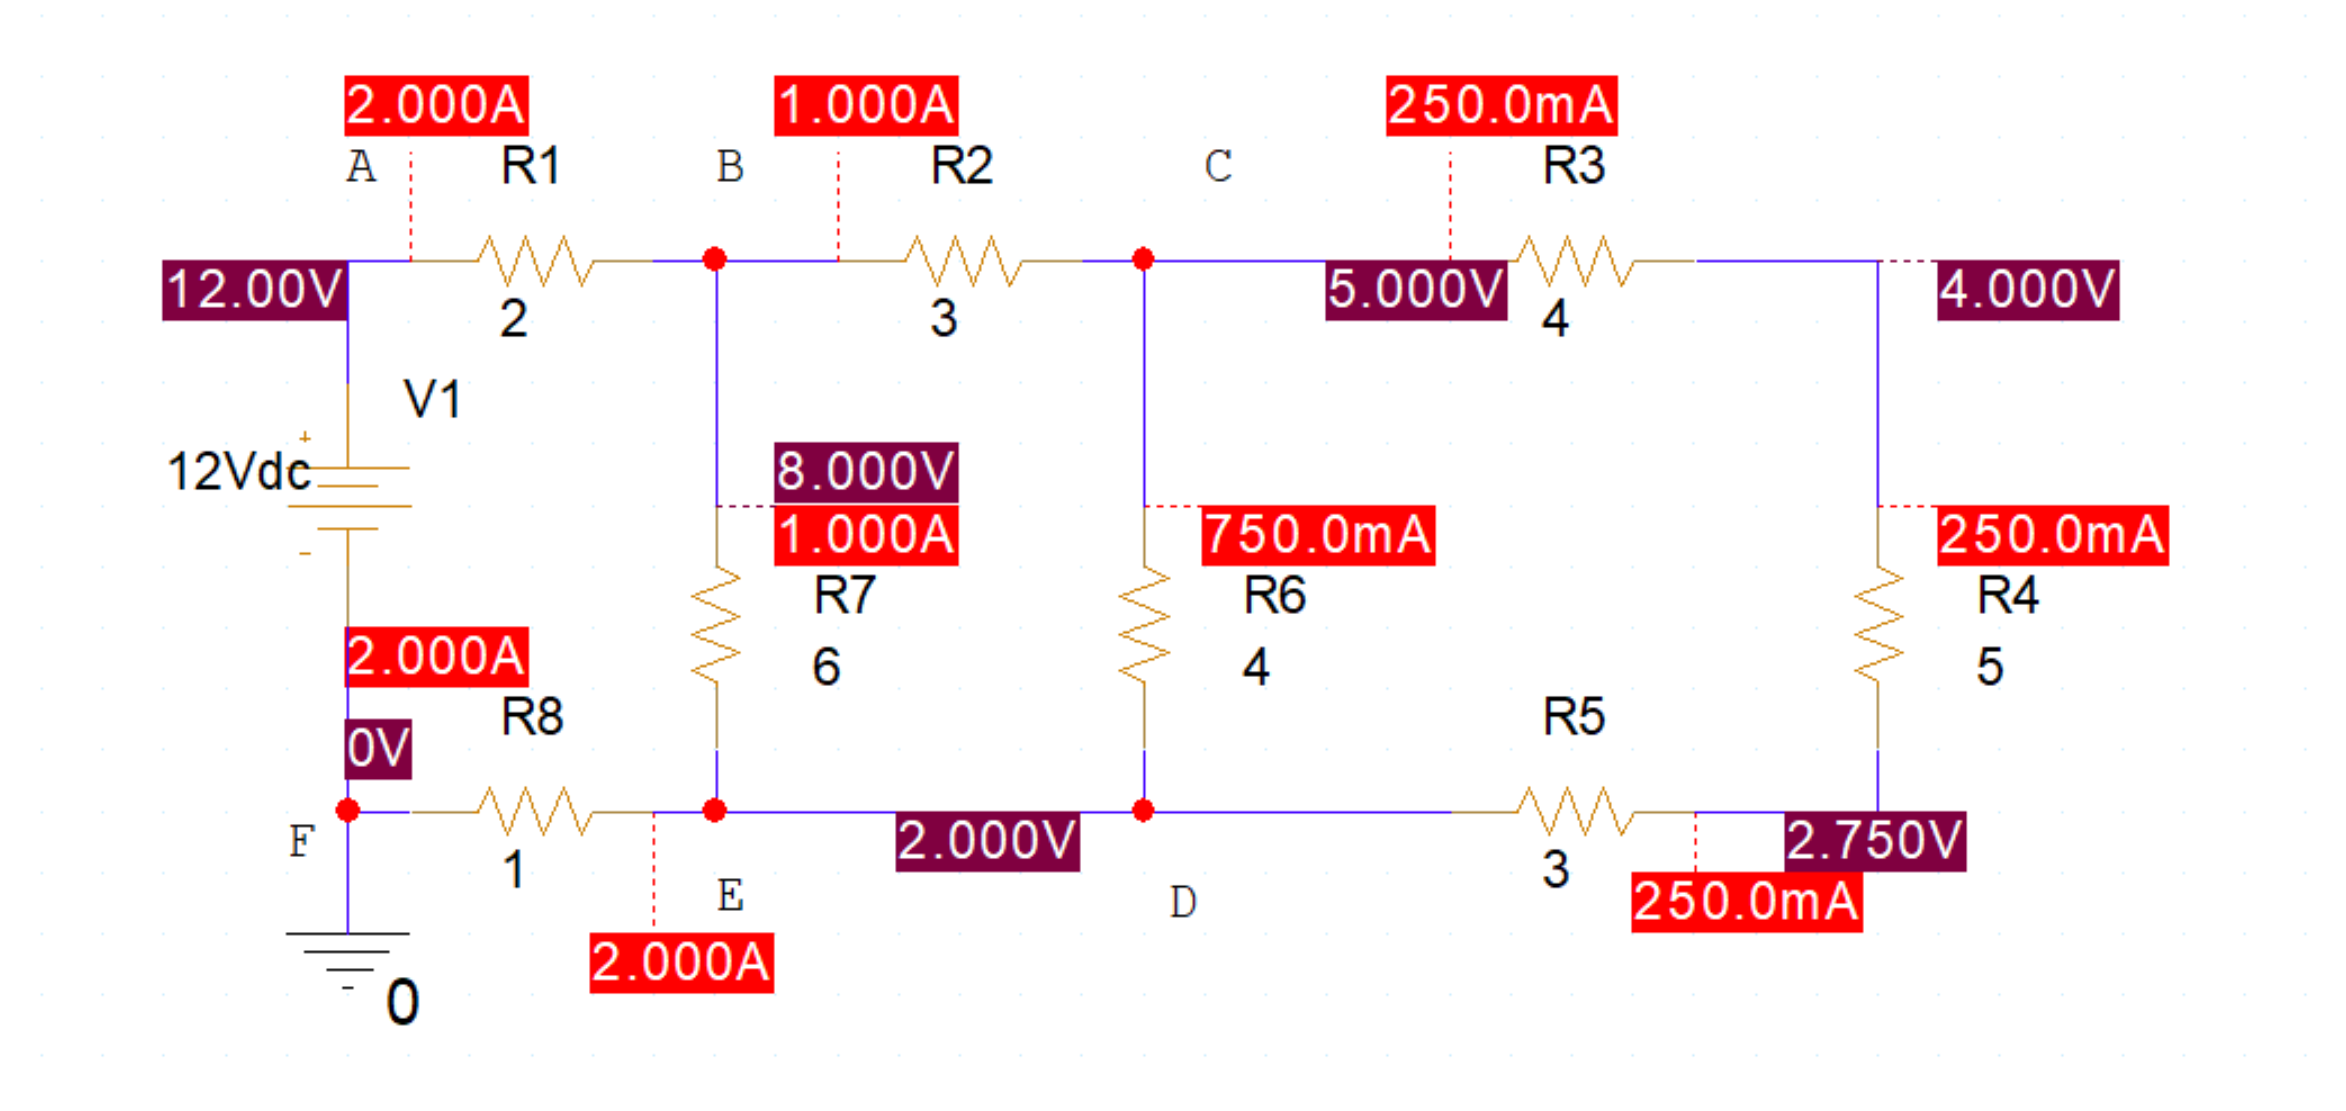
\includegraphics[width=1\textwidth]{graphics/ex2/f2.png}
    \caption{Mạch ban đầu}
    \end{figure}
    \begin{figure}[!htbp]
        \centering
        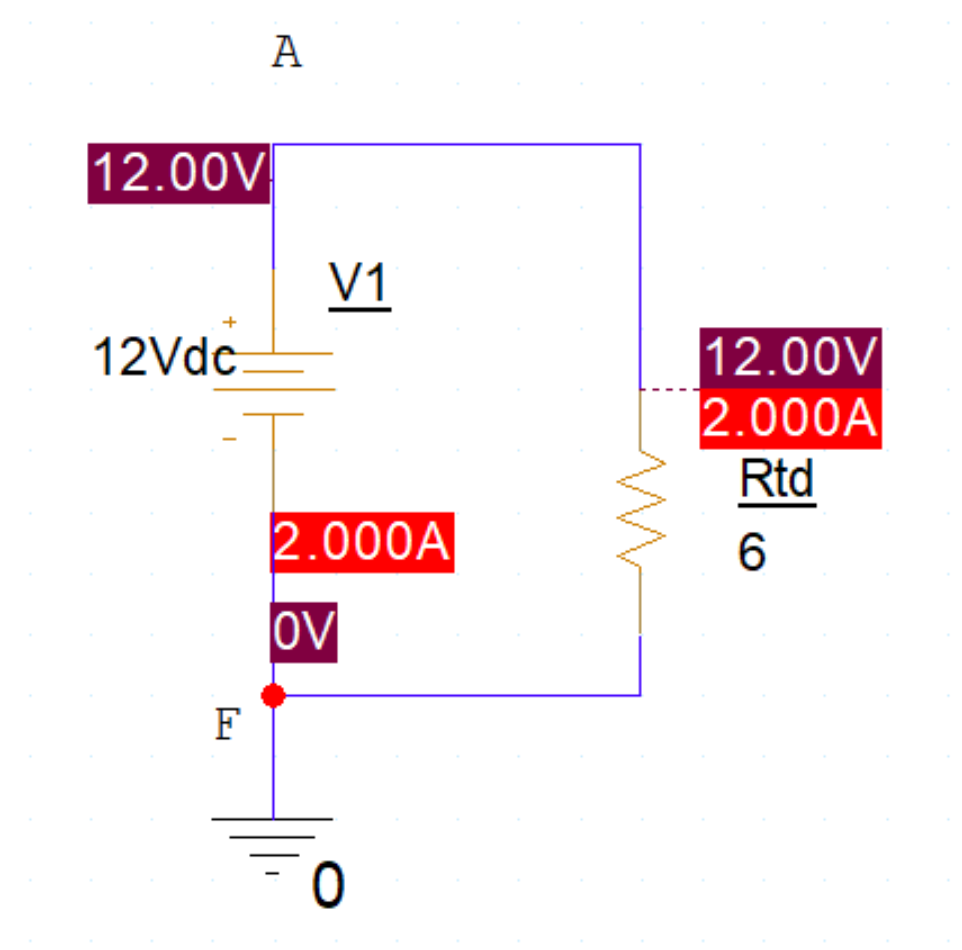
\includegraphics[width=0.5\textwidth]{graphics/ex2/f6.png}
        \caption{Mạch tương đương}
        \end{figure}

